%\documentclass[handout]{beamer}
\documentclass[lecture]{beamer}

\usepackage[latin1]{inputenc}
\usepackage{pifont,amsmath,amssymb,amsfonts,euscript,mathrsfs,wasysym,textcomp}
\usepackage{psfrag}
\usepackage{multimedia}
\usepackage{fancybox}
\usepackage{soul}
\usetheme{Boadilla}
\usepackage{xcolor}

\usepackage{array}
\usepackage{calc}

\usepackage{amsmath}

\setbeamertemplate{blocks}[rounded][shadow=false]

\newcommand {\cmatr}[2]{\left\{\begin{array}{#1}#2\end{array}\right.}

\makeatletter
\newcommand{\pushright}[1]{\ifmeasuring@#1\else\omit\hfill$\displaystyle#1$\fi\ignorespaces}
\newcommand{\pushleft}[1]{\ifmeasuring@#1\else\omit$\displaystyle#1$\hfill\fi\ignorespaces}
\makeatother

\DeclareMathOperator*{\argmax}{arg\,max}
\DeclareMathOperator*{\argmin}{arg\,min}



\newcommand{\highlightred}[1]{%
  \colorbox{red!50}{$\displaystyle#1$}}
  \newcommand{\highlightgreen}[1]{%
  \colorbox{green!50}{$\displaystyle#1$}}
\usepackage{pgfpages}
%\pgfpagesuselayout{4 on 1}[a4paper,landscape,border shrink=5mm]
%\pgfpagesuselayout{2 on 1}[letterpaper,border shrink=5mm]
\usepackage{mathtools}


\newtheorem{Proposition}{Proposition}

\usepackage{tikz}
\usetikzlibrary{arrows,shapes}
\tikzstyle{na} = [baseline=-.5ex]
\tikzstyle{every picture}+=[remember picture]
\usetikzlibrary{positioning,intersections}

\makeatletter
\def\hlinewd#1{%
\noalign{\ifnum0=`}\fi\hrule \@height #1 %
\futurelet\reserved@a\@xhline}
\makeatother



\newsavebox{\fmbox}
\newenvironment{fmpage}[1]
  {\begin{lrbox}{\fmbox}\begin{minipage}{#1}}
  {\end{minipage}\end{lrbox}\fbox{\usebox{\fmbox}}}

\newcommand\BackgroundPicture[1]{%
   \setbeamertemplate{background}{%
   \parbox[c][\paperheight]{\paperwidth}{%
       \vfill \hfill
        \includegraphics[width=1\paperwidth,height=1\paperheight]{#1}
        \hfill \vfill
}}}

\definecolor{myGreen}{rgb}{0.,0.4,0.}
\definecolor{myGreen2}{rgb}{0.,0.8,0.}
\definecolor{myGreen3}{rgb}{0.,0.6,0.}
\definecolor{myLightGreen}{rgb}{0.9,1,0.9}
\definecolor{myBlue}{rgb}{0.,0.,0.4}
\definecolor{myBlue2}{rgb}{0,0.1,0.8}
\definecolor{myOrange}{rgb}{1.,0.5,0.}
\definecolor{myBrown}{rgb}{.65,.16,.15}
\definecolor{myCyan}{rgb}{.65,.16,.15}
\definecolor{myPurple}{rgb}{1,0,1}
\definecolor{myRed}{rgb}{0.8,0,0}
\definecolor{myRed2}{rgb}{0.65,0,0}
\definecolor{deepBlue}{rgb}{0.0,0,1}

\definecolor{myLightBlue}{rgb}{0.9,0.9,1}
\definecolor{myLightRed}{rgb}{1,0.9,0.9}


\newcommand{\FSII}{1}
\newcommand{\FSIII}{0.8}




\newcommand {\condmatr}[2]{\left\{\begin{array}{#1}#2\end{array}\right.}
\newcommand{\defi}{\stackrel{\footnotesize\Delta}{=}}
\newcommand{\expon}[1]{\ensuremath{\textnormal{e}^{#1}}}
\newcommand{\RR}{\textnormal{\textsf{I}\!\textsf{R}}}
\newcommand{\ini}[1]{\ensuremath{#1_{k}}}
\newcommand{\fin}[1]{\ensuremath{#1_\textnormal{f}}}
\newcommand{\der}[1]{\textnormal{d}{#1}}
\newcommand{\derk}[2]{\textnormal{d}^{#1}#2}
\newcommand{\ddt}[1]{\frac{\der{#1}}{\der{t}}} 
\newcommand{\dkdtk}[2]{\frac{\derk{#1}{#2}}{\der{t}^{#1}}} 
\newcommand{\dd}[2]{\frac{\der{#1}}{\der{#2}}} 
\newcommand{\NN}{\ensuremath{\textnormal{\textsf{I}\!\textsf{N}}}}
\newcommand {\matr}[2]{\left[\begin{array}{#1}#2\end{array}\right]}
\newcommand {\omatr}[2]{\begin{array}{#1}#2\end{array}}
%\newcommand{\Rn}[1]{\ensuremath{\RR^{#1}}}
%\newcommand{\En}[1]{\ensuremath{E_{#1}}}
\newcommand{\En}[1]{\ensuremath{\RR^{#1}}}
\newcommand{\R}[1]{\ensuremath{\RR^{#1}}}
\newcommand{\lagr}{\ensuremath{\mathcal{L}}}
\newcommand{\hamil}{\ensuremath{\mathcal{H}}}
\newcommand{\hamax}{\ensuremath{\mathcal{M}}}
\newcommand{\ndxset}{\ensuremath{\EuScript{K}}}
\newcommand{\id}[1]{\ensuremath{I_{#1}}}
%\newcommand{\matr}[1]{\ensuremath{\textnormal{\sf #1}}}
\newcommand{\vect}[1]{\ensuremath{\boldsymbol{\mathrm{#1}}}}
\newcommand{\const}[1]{\ensuremath{\overline{#1}}}
\newcommand{\fixed}[1]{\ensuremath{\underline{#1}}}
\newcommand{\transp}[1]{\ensuremath{{#1}^\textnormal{\textsf{T}}}}
\newcommand{\invtr}[1]{\ensuremath{{#1}^{-\textnormal{\textsf{T}}}}}
\newcommand{\inv}[1]{\ensuremath{#1^{-1}}}
\newcommand{\inter}[1]{\ensuremath{\textnormal{int}\left({#1}\right)}}
\newcommand{\closur}[1]{\ensuremath{\textnormal{cl}\left({#1}\right)}}
\newcommand{\rank}[1]{\ensuremath{\oprank\left({#1}\right)}}
\newcommand{\diag}[1]{\ensuremath{\opdiag\left({#1}\right)}}
\renewcommand{\ker}[1]{\ensuremath{\opker\left({#1}\right)}}
\renewcommand{\det}[1]{\ensuremath{\opdet\left({#1}\right)}}
\newcommand{\opt}[1]{{#1}^\star}
\newcommand{\nom}[1]{{#1}^\star}
\newcommand{\pert}[1]{{#1}^\dagger}
\newcommand{\activ}[2]{\ensuremath{\EuScript{A}_{#1}\left(#2\right)}}
\newcommand{\ball}[2]{\ensuremath{\EuScript{B}_{#1}\left(#2\right)}}
\newcommand{\iball}[3]{\ensuremath{\EuScript{B}_{#1}^{#2}\left(#3\right)}}
\newcommand{\cball}[2]{\ensuremath{\bar{\EuScript{B}}_{#1}\left(#2\right)}}
\newcommand{\dball}[2]{\ensuremath{\dot{\EuScript{B}}_{#1}\left(#2\right)}}
\newcommand{\boun}[1]{\ensuremath{\partial #1}}
\newcommand{\C}[1]{\ensuremath{\mathcal{C}^{#1}}}
\newcommand{\PWC}[1]{\ensuremath{\hat{\mathcal{C}}^{#1}}}
\newcommand{\proj}[2]{\ensuremath{\mathcal{P}_{#1}#2}}
\newcommand{\F}{\ensuremath{\EuScript{F}}}
\newcommand{\J}{\ensuremath{\EuScript{J}}}
\newcommand{\D}{\ensuremath{\EuScript{D}}}
\newcommand{\X}{\ensuremath{\EuScript{X}}}
\newcommand{\K}{\ensuremath{\EuScript{K}}}
\newcommand{\U}{\ensuremath{\EuScript{U}}}
\newcommand{\V}{\ensuremath{\EuScript{V}}}
\renewcommand{\P}{\ensuremath{\EuScript{P}}}
\newcommand{\ext}[1]{\ensuremath{\tilde{#1}}}
\newcommand{\tang}{\ensuremath{\mathscr{T}}}
\newcommand{\impdir}[1]{\ensuremath{\mathscr{D}}(#1)}
\newcommand{\feasdir}[2]{\ensuremath{F}_{#1}\left(#2\right)}
%\newcommand{\activ}[1]{\ensuremath{\EuScript{A}(#1)}}
\newcommand{\dc}{c}
\newcommand{\RK}{\ensuremath{\textnormal{RK}}}

\newcommand{\intP}{\vect{P}}
\newcommand{\intXk}{X}
\newcommand{\intX}{\vect{\intXk}}
\newcommand{\x}{{\bf x}}
\newcommand{\y}{{\bf y}}
\newcommand{\p}{{\bf p}}
\newcommand{\q}{{\bf q}}
\newcommand{\term}{\phi}
\newcommand{\integ}{\psi}
\newcommand{\ODEi}{f}
\newcommand{\ODE}{\vect{\ODEi}}
\newcommand{\ODECVXi}[1]{u_{f_{#1}}}
\newcommand{\ODECVX}{\vect{\ODECVXi{}}}
\newcommand{\ODECCVi}[1]{o_{f_{#1}}}
\newcommand{\ODECCV}{\vect{\ODECCVi{}}}
\newcommand{\ICi}[1]{h_{#1}}
\newcommand{\IC}{\vect{\ICi{}}}
\newcommand{\ICCVXi}[1]{u_{h_{#1}}}
\newcommand{\ICCVX}{\vect{\ICCVXi{}}}
\newcommand{\ICCCVi}[1]{o_{h_{#1}}}
\newcommand{\ICCCV}{\vect{\ICCCVi{}}}

\newcommand{\lb}[1]{#1^{\rm L}}
\newcommand{\ub}[1]{#1^{\rm U}}
\newcommand{\cv}[1]{\vect{u}_{#1}}
\newcommand{\cc}[1]{\vect{o}_{#1}}
\newcommand{\dcv}[1]{\dot{\vect{u}}_{#1}}
\newcommand{\dcc}[1]{\dot{\vect{o}}_{#1}}
\newcommand{\cvi}[1]{u_{#1}}
\newcommand{\cci}[1]{o_{#1}}
\newcommand{\trace}[1]{\text{Tr}\left(#1\right)}

\DeclareMathOperator{\esssup}{ess\,sup}
\DeclareMathOperator{\essinf}{ess\,inf}
\DeclareMathOperator{\sign}{sign}
\DeclareMathOperator{\oprank}{rank}
\DeclareMathOperator{\opker}{ker}
\DeclareMathOperator{\opdet}{det}
\DeclareMathOperator{\opdiag}{diag}
\DeclareMathOperator{\midf}{mid}
\DeclareMathOperator{\opcard}{card}

\definecolor{myGreen}{rgb}{0.,0.4,0.}
\definecolor{myGreen2}{rgb}{0.,0.8,0.}
\definecolor{myGreen3}{rgb}{0.,0.6,0.}
\definecolor{myBlue}{rgb}{0.,0.,0.4}
\definecolor{myBlue2}{rgb}{0,0.1,0.8}
\definecolor{myOrange}{rgb}{1.,0.5,0.}
\definecolor{myOrange2}{rgb}{0.8.,0.5,0.}
\definecolor{myBrown}{rgb}{.65,.16,.15}
\definecolor{myCyan}{rgb}{.65,.16,.15}
\definecolor{myPurple}{rgb}{1,0,1}
\definecolor{myRed}{rgb}{0.8,0,0}

\usetikzlibrary{arrows,positioning,calc}

\usepackage[ruled,vlined]{algorithm2e}
\renewcommand{\thealgocf}{}
\newtheorem {Algorithm}{Algorithm}
\SetAlCapFnt{\scriptsize}
\usepackage{caption}

\usepackage{tikz}
\usetikzlibrary{positioning,arrows}
\AtBeginSection[]
{
{\usebackgroundtemplate{
 \parbox[c][\paperheight][b]{\paperwidth}{
    \flushright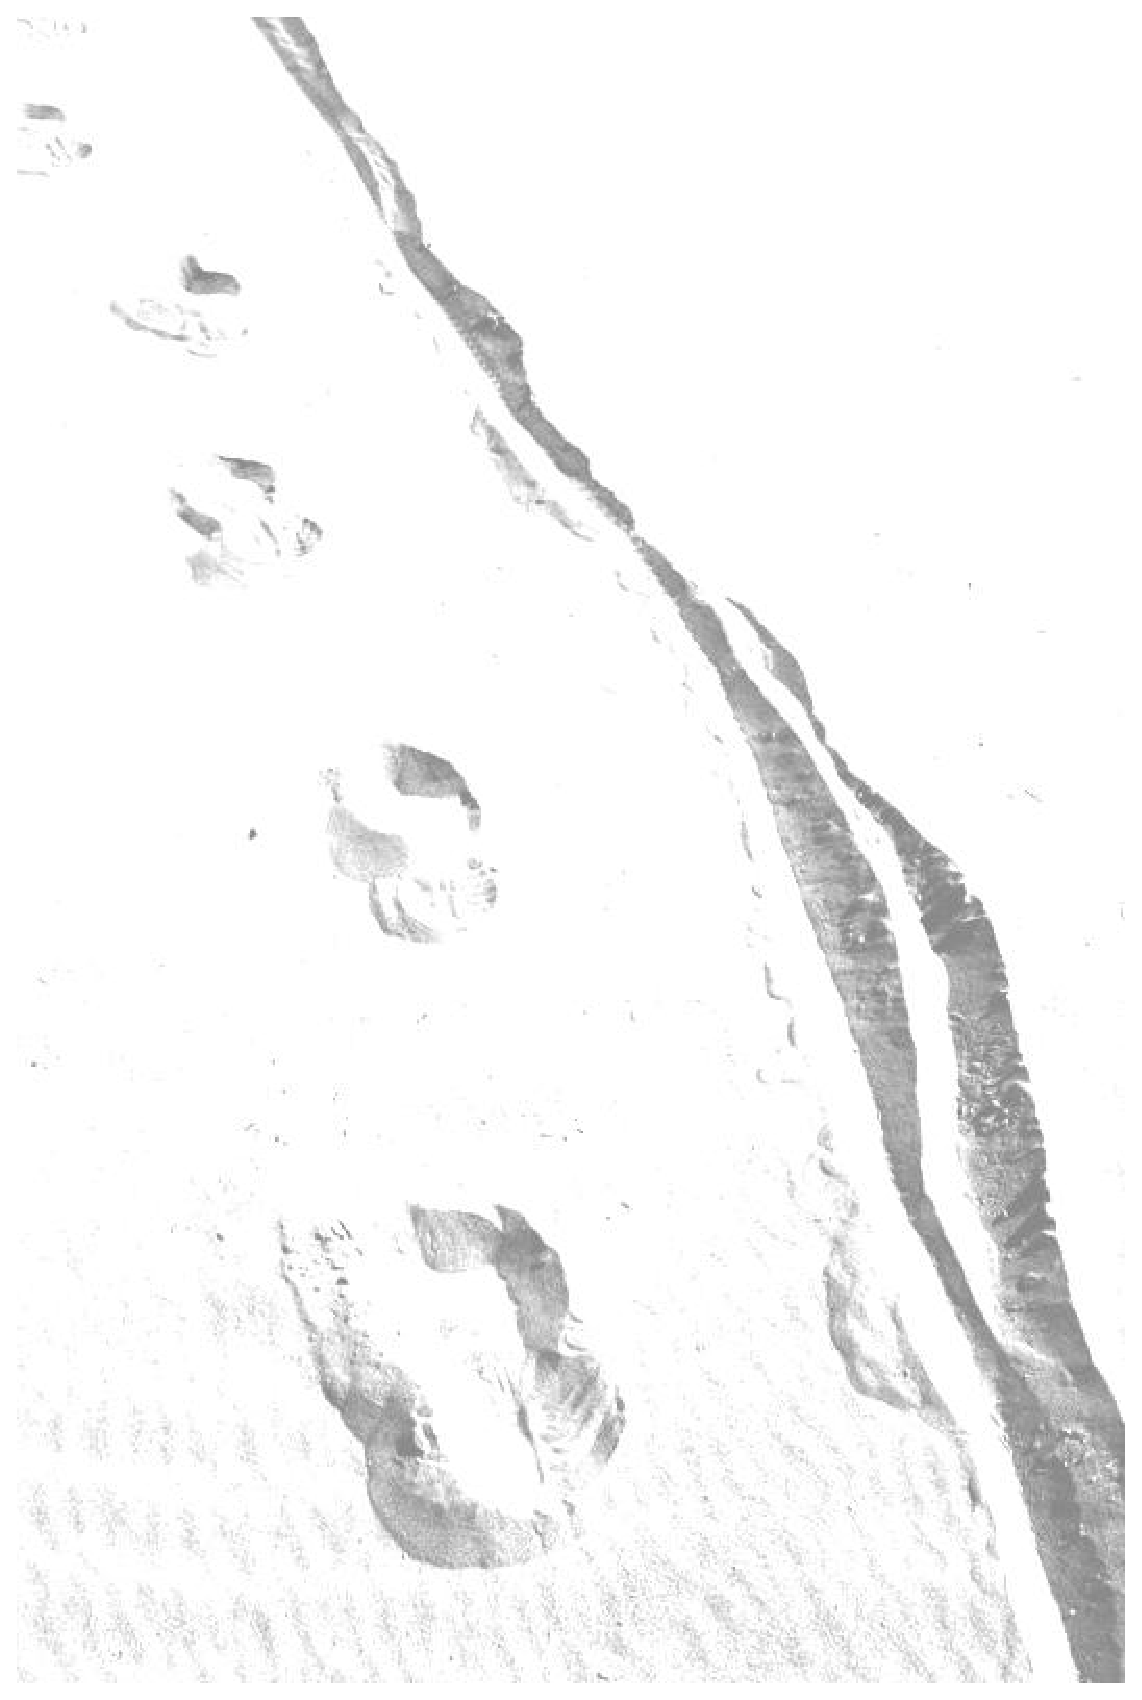
\includegraphics[width=0.55\paperwidth, height = \paperheight]{Figures/Track.eps}}}
  \begin{frame}{\normalsize Outline}
  \tableofcontents[currentsection]
  \end{frame}}
}



\title[RL-MPC]{Merging AI \& Optimization for Decision-Making\\
A Decision-Oriented Approach Using \\
Reinforcement Learning \& MPC
}
\author[S. Gros]{\large Sebastien Gros}
\institute[NTNU]{Department of Cybernetic \\ Faculty of Information Technology \\  NTNU}
\date[September 2025]{AI Wokshop 2025}

%%%%%%%%%%%%%%%%%%%%%%%%%%%%%%%%%%%%%%%%%%%%%%%%%%%%%%%%%%%%%%%%%%%%%%%%

\begin{document}




{\usebackgroundtemplate{
 \parbox[c][\paperheight][b]{\paperwidth}{
    \flushright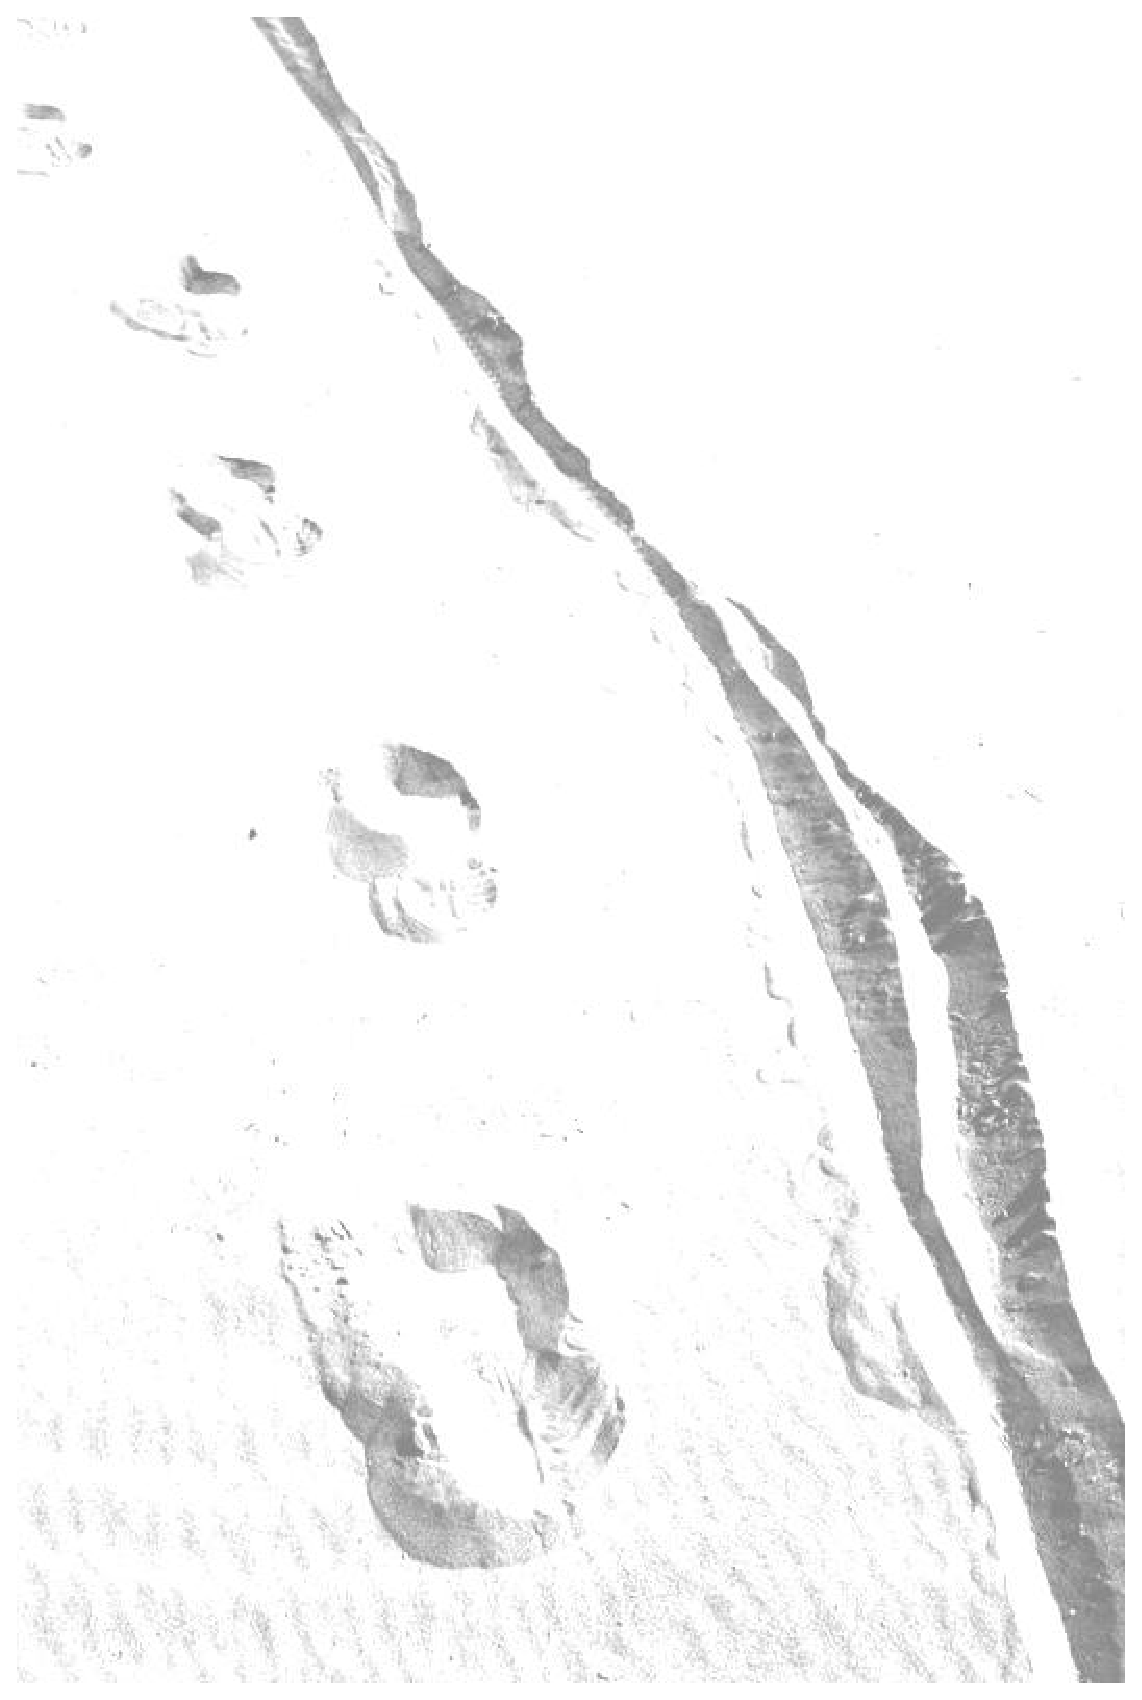
\includegraphics[width=0.55\paperwidth, height = 1\paperheight]{Figures/Track.eps}}}
\begin{frame}
\titlepage
\end{frame}}










\begin{frame}{\normalsize Policy From Repeated Planning - Model Predictive Control (MPC)}
\footnotesize
\begin{center}
\textbf{Optimize a plan over a finite horizon, apply first move, repeat}
\end{center}
\vspace{-.5cm}
\begin{columns}[t]
\column{0.45\textwidth}
\begin{block}{}
\textbf{MPC}: at {\color{blue}current state $\vect s$}
\vspace{-.4cm}\\
\begin{overlayarea}{\textwidth}{0.4\textheight}
\only<1-8>{
\begin{align*}
\max_{\text{action plan}}&\,  \sum_{\text{horizon}}\text{Utility}(\text{action},\text{prediction}) \\
\mathrm{s.t.}&\quad \text{action plan}\rightarrow \text{prediction}\\
&\quad \text{prediction starts at } {\color{blue}\vect s}\\
&\quad  \text{safety constraints } 
%\vect x_{k+1} = \vect f\left(\vect x_k,\vect u_k\right)\\
%&\quad  \vect h\left(\vect x_k,\vect u_k\right)\leq 0\\
%&\quad \vect{x}_0 = {\color{blue}\vect s}
\end{align*}
apply {\color{myGreen3}first action of the plan} 
}
\only<9->{
\begin{align*}
\max_{\vect x,{\color{myGreen3}\vect u}}&\quad T\left(\vect x_N\right) +  \sum_{k=0}^{N-1} L\left(\vect x_k,\vect u_k\right)  \\
\mathrm{s.t.}&\quad \vect x_{k+1} = \vect f\left(\vect x_k,\vect u_k\right)\\
&\quad  \vect h\left(\vect x_k,\vect u_k\right)\leq 0\\
&\quad \vect{x}_0 = {\color{blue}\vect s}
\end{align*}
apply {\color{myGreen3}action $\vect a = \vect u_0^\star$} to the system
}
\end{overlayarea}
\end{block}

\column{0.55\textwidth}
\begin{figure}
\newcommand{\FS}{.8}
\psfrag{x}[Bl][Bl][1]{$\textcolor{blue}{\vect{s}}$}
\psfrag{t}[Bl][Bl][.7]{Current time}
\psfrag{pi}[Bl][Bl][1]{$\vect{\pi}(\textcolor{blue}{\vect{s}})$}
\includegraphics<1>[width=\FS\textwidth,clip]{Figures/MPC0.eps}
\includegraphics<2>[width=\FS\textwidth,clip]{Figures/MPC1.eps}
\includegraphics<3>[width=\FS\textwidth,clip]{Figures/MPC2.eps}
\includegraphics<4>[width=\FS\textwidth,clip]{Figures/MPC3.eps}
\includegraphics<5>[width=\FS\textwidth,clip]{Figures/MPC4.eps}
\includegraphics<6>[width=\FS\textwidth,clip]{Figures/MPC5.eps}
\includegraphics<7>[width=\FS\textwidth,clip]{Figures/MPC6.eps}
\includegraphics<8->[width=\FS\textwidth,clip]{Figures/MPC7.eps}
%\includegraphics<11->[width=\FS\textwidth,clip]{Figures/Hybrid.eps}
\end{figure}
\end{columns}

\vspace{-.5cm}

\begin{columns}
\column{0.45\textwidth}
\visible<10->{
\begin{block}{}
\textbf{MPC} 
\begin{itemize}
\item is \textbf{repeated planning}
\item implicitly it defines a \textbf{policy} $${\color{myGreen3}\vect a} = \vect\pi^\mathrm{MPC}\left({\color{blue}\vect s}\right) = \vect u^\star_{0} = \text{first action}
$$
\end{itemize}}
\end{block}

\column{0.5\textwidth}

\begin{overlayarea}{\textwidth}{0.25\textheight}
\only<9-10>{
\begin{itemize}
\item $\vect u_{0,\ldots,N-1}$: action plan
\item $\vect x_{0,\ldots,N}$: model-based predictions
\end{itemize} 
}
\only<11>{
\begin{alertblock}{}
\center
\textbf{You can replace ``MPC" any decision making from repeated planning (OR, CO, MSSP, MPPI, etc. This is ``classical" optimization-based decision making)
}
\end{alertblock}
}
\only<12>{
\begin{alertblock}{}
\center
\textbf{
In the presence of stochasticity \& model inaccuracy: intricate relationship between ``planning" and ``policing"}
\end{alertblock}
}
\end{overlayarea}

\end{columns}

\end{frame}


%
%\begin{frame}{\normalsize Theoretical Framework} % - Markov Decision Processes (MDPs)
%\footnotesize
%
%\begin{center}
%\visible<2->{\textbf{Connecting RL and MPC?}}
%\end{center}
%%\newcommand{\Sys}{\vspace{-0.25cm}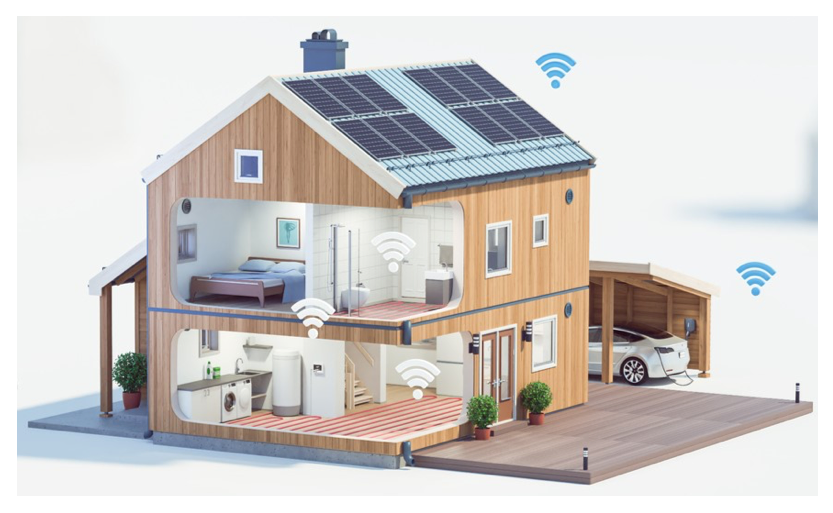
\includegraphics[width=1\textwidth,clip]{Figures/SmartHouse.eps}}
%
%\tikzstyle{MPC_block} = [rectangle, draw, fill=myLightRed,  text width=4cm, text centered, rounded corners, minimum height=4em,inner sep=2pt]
%\tikzstyle{MDP_block} = [rectangle, draw, fill=myLightGreen,  text width=7.5cm,  text centered, rounded corners, minimum height=4em,inner sep=2pt]
%\tikzstyle{RL_block} = [rectangle, draw, fill=myLightBlue,  text width=5cm, text centered, rounded corners, minimum height=4em,inner sep=2pt]    
%\tikzstyle{line} = [draw, -latex',<->]
%
%\begin{tikzpicture}%[node distance = 4cm, auto]
%
%\visible<3->{
%\node [MDP_block] (MDP0) {
% \begin{minipage}[c]{7.5cm}
%\textbf{\,Markov Decision Process (MDP)}
%\begin{itemize}
%\item Framework to understand optimal policies
%\item Dynamics assumed stochastic ``by default"
%\item Very permissive, Bellman equations
%%\item Powerful abstraction of real-world problems
%\end{itemize} 
%\end{minipage}
% };}
% 
% 
%\node [MPC_block, left of=MDP0, above of=MDP0, node distance = 3.5cm] (MPC0) {
% \begin{minipage}[c]{4cm}
%\textbf{\,Model Predictive Control}
%\begin{itemize}
%\item Control tool
%\item Policies from planning
%\item Explicit predictions
%\end{itemize} 
%\end{minipage}
%};
%
% 
%\node [RL_block, right of=MDP0, above of=MDP0, node distance = 3.5cm] (RL0) {
% \begin{minipage}[c]{5cm}
% \textbf{\,Reinforcement Learning (RL)}
%\begin{itemize}
%\item Toolbox
%\item Optimal policies from learning
%\item No explicit prediction
%\end{itemize} 
%\end{minipage}
% };
% 
%\visible<4->{\path [line] (RL0) -- node [ anchor=west] {\,\, \textcolor{myGreen}{Solves MDP from data}} (MDP0);}
%\visible<5->{\path [line] (MDP0) -- node [ anchor=east] {\textcolor{blue}{Connection?}\,\,} (MPC0);}
%\visible<2->{\path [line] (MPC0) -- node [ anchor=south] {\textcolor{myRed}{Connection?}} (RL0);}
%
%\end{tikzpicture}
%\center
%\visible<6->{\textbf{RL for MPC consists first in understanding MPC \& MDPs}}
%
%\end{frame}

%\section{The Basics}





%
%
%\begin{frame}{\normalsize Optimal policies? }
%\footnotesize
%
%
%
%\begin{columns}[t]
%\column{0.49\textwidth}
%\visible<2->{
%\begin{alertblock}{}
%\textbf{MDP optimality cast as} minimizing$^\dagger$
%\begin{align*}
%\visible<7->{J\left(\vect \pi \right) =} \visible<6->{\mathbb E\left[}\left. \visible<3->{\sum_{k=0}^\infty}  \visible<5->{\gamma^k} \visible<3->{L\left(\vect s_k,\vect a_k\right)} \visible<4->{\,\right|\, \vect a_k = \vect\pi\left(\vect s_k\right)} \visible<6->{ \right]}
%\end{align*}
%\flushright \visible<5->{with discount $0<\gamma<1$}
%\end{alertblock}}
%\vspace{-.25cm}
%\begin{block}{}
%\textbf{MPC} policy  $\vect\pi^\mathrm{MPC}\left({\color{blue}\vect s}\right) = {\color{myGreen3}\vect u^\star_{0}}$ from
%\vspace{-.5cm}\\
%\begin{align*}
%\min_{\vect x,\vect u}&\quad   T\left(\vect x_N\right) + \sum_{k=0}^{N-1} L\left(\vect x_k,\vect u_k\right)  \\
%\mathrm{s.t.}&\quad \vect x_{k+1} = \vect f\left(\vect x_k,\vect u_k\right)\\
%&\quad  \vect h\left(\vect x_k,\vect u_k\right)\leq 0\\
%&\quad \vect{x}_0 = {\color{blue}\vect s}
%\end{align*}
%\end{block}
%
%\visible<13->{
%\begin{alertblock}{}
%\center
%\textbf{Can learning help with that?}
%\end{alertblock}
%}
%
%
%
%\column{0.02\textwidth}
%\column{0.49\textwidth}
%\vspace{-1.25cm}
%\newcommand{\FS}{.8}
%\begin{figure}
%\psfrag{x}[Bl][Bl][1]{$\textcolor{blue}{\vect{s}}$}
%\psfrag{t}[Bl][Bl][.7]{Current time}
%\psfrag{pi}[Bl][Bl][1]{$\vect{\pi}(\textcolor{blue}{\vect{s}})$}
%\includegraphics<1->[width=\FS\textwidth,clip]{Figures/SimpleTrajectories8.eps}
%\end{figure}
%
%\vspace{-.6cm}
%
%\visible<8->{
%\begin{block}{}
%Optimal policy $ \vect\pi^\star$:
%\begin{align*}
%\vect\pi^\star = \mathrm a\min_{\vect\pi}\,\, J\left(\vect \pi \right)
%\end{align*}
%\end{block}}
%
%\begin{overlayarea}{\textwidth}{0.6\textheight}
%\only<9-11>{
%\begin{alertblock}{}
%\scriptsize
%\center
%$^\dagger$\textbf{Alternatives}: finite horizon, conditional termination, undiscounted, beyond 1$^\mathrm{st}$ moment
%\end{alertblock}
%
%\visible<10->{$^\dagger$ Also sometimes presented as criteria in MPC literature (without discount)} 
%
%\visible<11->{\center \textit{Note: MDP puts the constraints with the cost, dissmissed here for simplicity} 
%}
%}
%
%\only<12->{\begin{block}{}
%\textbf{Does MPC give} $\vect\pi^\mathrm{MPC}= \vect\pi^\star$?
%\visible<13->{
%\begin{enumerate}
%\item Infinite vs. finite horizon 
%\item Discounted ($\gamma<1$) vs. undiscounted
%\item \textbf{Model $\vect f$ \textcolor{myRed2}{inaccurate}}
%\end{enumerate} }
%\flushright \textbf{... in general no}
%\end{block}}
%\end{overlayarea}
%
%
%
%\end{columns}
%
%
%
%\end{frame}



%
%\begin{frame}{\normalsize Optimal policies? }
%\footnotesize
%
%\begin{overlayarea}{\textwidth}{\textheight}
%\only<1>{
%
%\begin{columns}
%\column{0.475\textwidth}
%\begin{alertblock}{}
%\center
%\textcolor{myBlue2}{\textbf{Tracking MPC}}\\
%Historically MPC focuses on \textbf{constraints satisfaction \& stability}. Cost for reference tracking.
%\end{alertblock} 
%\column{0.475\textwidth}
%\begin{alertblock}{}
%\center
%\textcolor{myBlue2}{\textbf{Economic MPC}}\\
%More recently, focus on \textbf{closed-loop performance}, e.g. energy, time, money. Cost is generic.
%\end{alertblock} 
%\end{columns}
%\vspace{0.5cm} 
%\begin{columns}
%\column{0.2\textwidth}
%
%\column{0.6\textwidth}
%\center
%\textbf{The concept of optimal policy takes its full sense if cost to minimize has a meaning} 
%
%\column{0.2\textwidth}
%\end{columns}
%
%}
%
%\only<2->{
%
%\begin{columns}[t]
%\column{0.49\textwidth}
%\visible<2->{
%\begin{alertblock}{}
%\textbf{MDP optimality cast as} minimizing$^\dagger$
%\begin{align*}
%\visible<7->{J\left(\vect \pi \right) =} \visible<6->{\mathbb E\left[}\left. \visible<3->{\sum_{k=0}^\infty}  \visible<5->{\gamma^k} \visible<3->{L\left(\vect s_k,\vect a_k\right)} \visible<4->{\,\right|\, \vect a_k = \vect\pi\left(\vect s_k\right)} \visible<6->{ \right]}
%\end{align*}
%\flushright \visible<5->{with discount $0<\gamma<1$}
%\end{alertblock}}
%\vspace{-.25cm}
%\begin{block}{}
%\textbf{MPC} policy  $\vect\pi^\mathrm{MPC}\left({\color{blue}\vect s}\right) = {\color{myGreen3}\vect u^\star_{0}}$ from
%\vspace{-.5cm}\\
%\begin{align*}
%\min_{\vect x,\vect u}&\quad   T\left(\vect x_N\right) + \sum_{k=0}^{N-1} L\left(\vect x_k,\vect u_k\right)  \\
%\mathrm{s.t.}&\quad \vect x_{k+1} = \vect f\left(\vect x_k,\vect u_k\right)\\
%&\quad  \vect h\left(\vect x_k,\vect u_k\right)\leq 0\\
%&\quad \vect{x}_0 = {\color{blue}\vect s}
%\end{align*}
%\end{block}
%
%\visible<13->{
%\begin{alertblock}{}
%\center
%\textbf{Can learning help with that?}
%\end{alertblock}
%}
%
%
%
%\column{0.02\textwidth}
%\column{0.49\textwidth}
%\vspace{-1.25cm}
%\newcommand{\FS}{.8}
%\begin{figure}
%\psfrag{x}[Bl][Bl][1]{$\textcolor{blue}{\vect{s}}$}
%\psfrag{t}[Bl][Bl][.7]{Current time}
%\psfrag{pi}[Bl][Bl][1]{$\vect{\pi}(\textcolor{blue}{\vect{s}})$}
%\includegraphics<1->[width=\FS\textwidth,clip]{Figures/SimpleTrajectories8.eps}
%\end{figure}
%
%\vspace{-.6cm}
%
%\visible<8->{
%\begin{block}{}
%Optimal policy $ \vect\pi^\star$:
%\begin{align*}
%\vect\pi^\star = \mathrm a\min_{\vect\pi}\,\, J\left(\vect \pi \right)
%\end{align*}
%\end{block}}
%
%\begin{overlayarea}{\textwidth}{0.6\textheight}
%\only<9-10>{
%\begin{alertblock}{}
%\scriptsize
%\center
%$^\dagger$\textbf{Alternatives}: finite horizon, conditional termination, bias optimal, gain optimal, beyond 1$^\mathrm{st}$ moment
%\end{alertblock}
%
%\visible<10->{\center \textit{Note: MDP puts the constraints with the cost} 
%}
%}
%
%\only<11->{\begin{block}{}
%\textbf{Does MPC give} $\vect\pi^\mathrm{MPC}= \vect\pi^\star$?
%\visible<12->{
%\begin{enumerate}
%\item Infinite vs. finite horizon 
%\item Discounted ($\gamma<1$) vs. undiscounted
%\item \textbf{Model $\vect f$ \textcolor{myRed2}{inaccurate}}
%\end{enumerate} }
%\flushright \textbf{... in general no}
%\end{block}}
%\end{overlayarea}
%
%
%
%\end{columns}}
%
%\end{overlayarea}
%
%
%
%\end{frame}
%


\begin{frame}{\normalsize Learning for MPC - Machine Learning for the Model}
\footnotesize

\newcommand{\Sys}{\vspace{-0.25cm}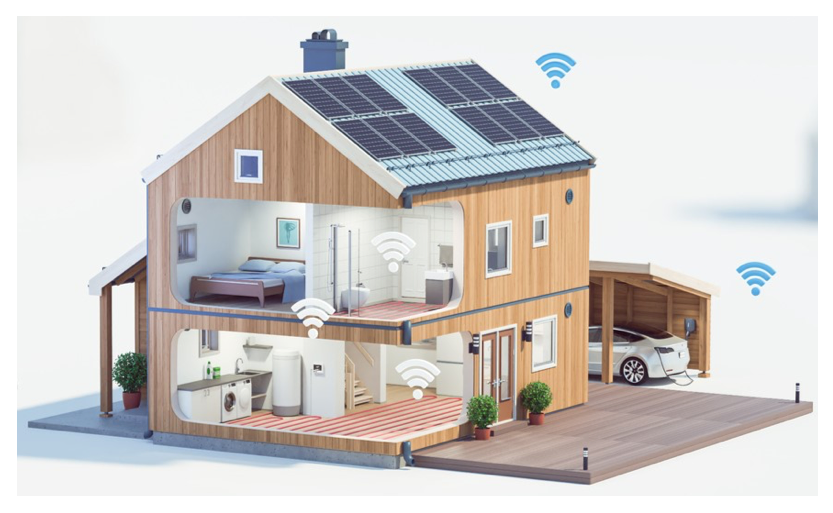
\includegraphics[width=1\textwidth,clip]{Figures/SmartHouse.eps}}

\tikzstyle{Sys_block} = [rectangle, draw, fill=none,  text width=3.cm, text centered, rounded corners, minimum height=4em,inner sep=2pt]
\tikzstyle{Opt_block} = [rectangle, draw, fill=myLightGreen,  text width=2.85cm,  text centered, rounded corners]
\tikzstyle{ID_block} = [rectangle, draw, fill=myLightBlue,  text width=3cm, text centered, rounded corners]    
\tikzstyle{line} = [draw, -latex']

\begin{tikzpicture}%[node distance = 4cm, auto]

\node [Sys_block] (sys0) {\Sys};
\node [Opt_block, left of=sys0, node distance = 4cm] (opt0) {
 \begin{minipage}[c]{2.75cm}
 \center
\textbf{MPC policy}
 \vspace{-0.1cm}
\begin{align*}
\vect\pi^\mathrm{MPC}_{\vect \theta}(\vect{s})
\end{align*}
\textbf{from model, e.g.}
\begin{align*}
\vect{x}_{k+1} = \vect{f}_{\vect{\theta}}(\vect{x}_k,\vect{u}_k)
\end{align*}
\end{minipage}
 };
 
\visible<2->{\node [ID_block, right of=sys0, node distance = 4.5cm] (ID0) {
 \begin{minipage}[c]{3.25cm}
\textbf{Machine-Learning}
\vspace{.2cm}\\
adjust ${\vect{\theta}}$ to fit model
\begin{align*}
\vect{s}_{k+1} = \vect{f}_{\vect{\theta}}(\vect{s}_k,\vect{a}_k)
\end{align*}
to data $\vect{s}_k,\vect{a}_k,\vect{s}_{k+1}$
\end{minipage}
 };}
\path [line] (opt0) -- node [ anchor=south] {$\vect{a}$} (sys0);
\path [line] (sys0.south)  -- ++(0,-0.5) -| node [ anchor=north] {$\vect{s}$} (opt0.south);
\visible<2->{\path [line] (sys0) -- node [ anchor=south] {$\vect{s}_+,\vect{s},\vect{a}$} (ID0);}
\visible<2->{\path [line] (ID0.north) -- ++(0,0.5) -| node [ anchor=south] {${\vect{\theta}}$} (opt0.north);}
 \end{tikzpicture}
 
%\vspace{-0.5cm}


\visible<3->{ 
\begin{columns}
\column{0.55\textwidth}
\textbf{``Machine Learning" in-the-loop} $\vect{f}_{\vect{\theta}}$ 
\begin{itemize}
\item \textbf{Physics-based}: first principles + SYSID
\item \textbf{Black-box linear}: ARX, SPC, etc.
\item  \textbf{Neural Network}: DNN, LSTM, TFT, $\ldots$
\item  \textbf{Statistical}: GP, GPC, RKHS, $\ldots$
\end{itemize}
%\visible<5->{\flushright \textbf{...same story for input-output models}}
}
\column{0.45\textwidth}
\vspace{-0.3cm}
\visible<4->{
\begin{alertblock}{}%\footnotesize \textbf{\textcolor{black}{Paradigm}}}
\textbf{\textcolor{black}{Defines a paradigm}}...\\
\vspace{0.1cm}
\visible<5->{
\begin{itemize}
\item Performance from model accuracy
%\item Target accuracy via ML
\item ``Ignore" that MPC is a policy
\end{itemize}}
\vspace{-.2cm} 
\flushright\textit{...in the context of optimal policies}
\end{alertblock}}
\vspace{-0.25cm}
\visible<6->{
\begin{block}{}
\center
\textbf{The focus of RL \& MPC is on offering another paradigm}
\end{block}


}
\end{columns}


\end{frame}


\begin{frame}{\normalsize Two Paradigm Shifts}
\footnotesize

\begin{columns}
\column{0.05\textwidth}
\column{0.85\textwidth}
\visible<2->{
\begin{alertblock}{}
%{\color{myBlue2}
\textbf{Shift 1: focus on performance instead of model fitting}
%}
\begin{itemize}
\item \textcolor{myRed}{\textbf{from}}: $\vect f_{\vect\theta}$ is a model for the system dynamics 
\item \textcolor{myBlue2}{\textbf{to}}: \quad MPC is a \textbf{model of the MDP solution}
\end{itemize}
\end{alertblock}}
\column{0.1\textwidth}
\end{columns}
\vspace{.25cm}
\begin{columns}[t]
\column{0.35\textwidth}
\visible<3->{
From \textcolor{myRed}{\textbf{classic}} view...
\begin{block}{}
\textbf{MPC}: at current state {\color{blue}$\vect s$} solve
\vspace{-.5cm}\\

\begin{align*}
\min_{\vect x,\vect u}&\quad   T\left(\vect x_N\right) + \sum_{k=0}^{N-1} L\left(\vect x_k,\vect u_k\right)  \\
\mathrm{s.t.}&\quad \vect x_{k+1} = \vect f_{\textcolor{myGreen3}{\vect\theta}}\left(\vect x_k,\vect u_k\right)\\
&\quad  \vect h\left(\vect x_k,\vect u_k\right)\leq 0\\
&\quad \vect{x}_0 = {\color{blue}\vect s}
\end{align*}
\flushright gives policy  $\vect\pi_{\textcolor{myGreen3}{\vect\theta}}^\mathrm{MPC}\left({\color{blue}\vect s} \right) = {\vect u^\star_{0}}$
\end{block}
\center
\textbf{
Find ${\textcolor{myGreen3}{\vect\theta}}$ such that prediction ``fits" the data}}
\column{0.01\textwidth}
\column{0.55\textwidth}
\visible<4->{
\textcolor{myBlue2}{\textbf{Shift to}...}\\
\center
\vspace{-0.1cm}
\textbf{
Find ${\textcolor{myGreen3}{\vect\theta}}$ that ``fits MPC to optimality" according to the data}{\scriptsize , e.g. minimizes $J\left(\vect\pi_{\textcolor{myGreen3}{\vect\theta}}^\mathrm{MPC}\right)$}}

\begin{overlayarea}{\textwidth}{0.6\textheight}
\only<5>{
\begin{itemize}
\item From model that best fits the data
\item To model for best closed-loop performance
%\item RL is a toolbox to do that...
\end{itemize}
\flushright ...but this may place a high demand on $ \vect f_{\textcolor{myGreen3}{\vect\theta}}$
%\vspace{0.5cm}
%\visible<6->{\textit{But getting $\vect\pi^\star$ places ``high demands" on $\vect f_{\textcolor{myGreen3}{\vect\theta}}$}} \\ %still may not get optimal policy} $\vect\pi^\star$...
%\flushright \visible<7->{Can we do more? \textcolor{myBlue2}{\textbf{Yes}}...}
}

\only<6>{
\vspace{-.5cm}
\begin{alertblock}{}
%{\color{myBlue2}
\textbf{Shift 2: full parametrization}%}
\vspace{-.5cm}\\
\begin{align*}
\min_{\vect x,\vect u}&\quad   T_{\textcolor{myGreen3}{\vect\theta}}\left(\vect x_N\right) + \sum_{k=0}^{N-1} L_{\textcolor{myGreen3}{\vect\theta}}\left(\vect x_k,\vect u_k\right)  \\
\mathrm{s.t.}&\quad \vect x_{k+1} = \vect f_{\textcolor{myGreen3}{\vect\theta}}\left(\vect x_k,\vect u_k\right)\\
&\quad  \vect h_{\textcolor{myGreen3}{\vect\theta}}\left(\vect x_k,\vect u_k\right)\leq 0\\
&\quad \vect{x}_0 = {\color{blue}\vect s}
\end{align*}
\vspace{-1cm}
\flushright gives policy  $\vect\pi_{\textcolor{myGreen3}{\vect\theta}}^\mathrm{MPC}\left({\color{blue}\vect s} \right) = {\vect u^\star_{0}}$
\end{alertblock}
\vspace{-.35cm}
\center
\textbf{MPC \textcolor{myRed}{built around} a model $\rightarrow$\\  MPC \textcolor{myRed}{is} a model}
}

\only<7>{
\vspace{0.0cm}
\center
\textbf{Is this idea justified?}  \textcolor{blue}{Yes...}
\begin{block}{}
\center
Under \textbf{\textcolor{blue}{some conditions}}, there is a $\textcolor{myGreen3}{\vect\theta}$ such that policy $ \vect\pi_{\textcolor{myGreen3}{\vect\theta}}^\mathrm{MPC}\left({\color{blue}\vect s} \right)$ is optimal in the real world
%\textbf{\textcolor{blue}{solves the MDP}}, even if model $\vect f_{\textcolor{myGreen3}{\vect\theta}}$ is inaccurate
\end{block}}
\end{overlayarea}

\end{columns}

\end{frame}


\begin{frame}{\normalsize Reinforcement Learning \& MPC }
\footnotesize

\begin{overlayarea}{\textwidth}{0.05\textheight}
\only<1>{
\center
\textbf{Classical Reinforcement Learning}
}
\only<2->{
\center
\textbf{Reinforcement Learning over MPC}
}
\end{overlayarea}
\vspace{-.5cm}
\newcommand{\Sys}{\vspace{-0.25cm}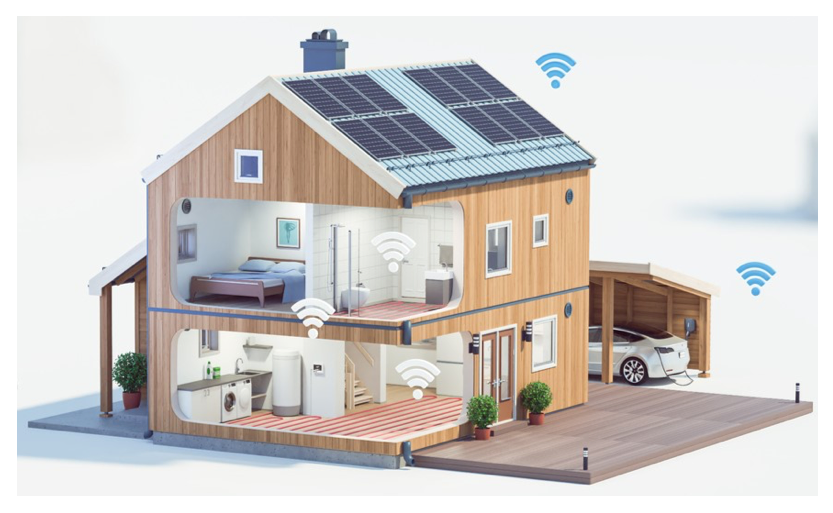
\includegraphics[width=1\textwidth,clip]{Figures/SmartHouse.eps}}

\tikzstyle{Sys_block} = [rectangle, draw, fill=none,  text width=2.5cm, text centered, rounded corners, minimum height=4em,inner sep=2pt]
\tikzstyle{Opt_block} = [rectangle, draw, fill=myLightGreen,  text width=3.5cm,  text centered, rounded corners]
\tikzstyle{ID_block} = [rectangle, draw, fill=myLightBlue,  text width=3.5cm, text centered, rounded corners]    
\tikzstyle{line} = [draw, -latex']

\begin{tikzpicture}%[node distance = 4cm, auto]

\node [Sys_block] (sys0) {\Sys};

\node [Opt_block, left of=sys0, node distance = 4cm] (opt0) {
\begin{overlayarea}{\textwidth}{0.325\textheight}
\only<1>{\center
  $\vect\pi_{\textcolor{myGreen3}{\vect\theta}}$ given by
  \vspace{-.15cm}
\begin{figure}
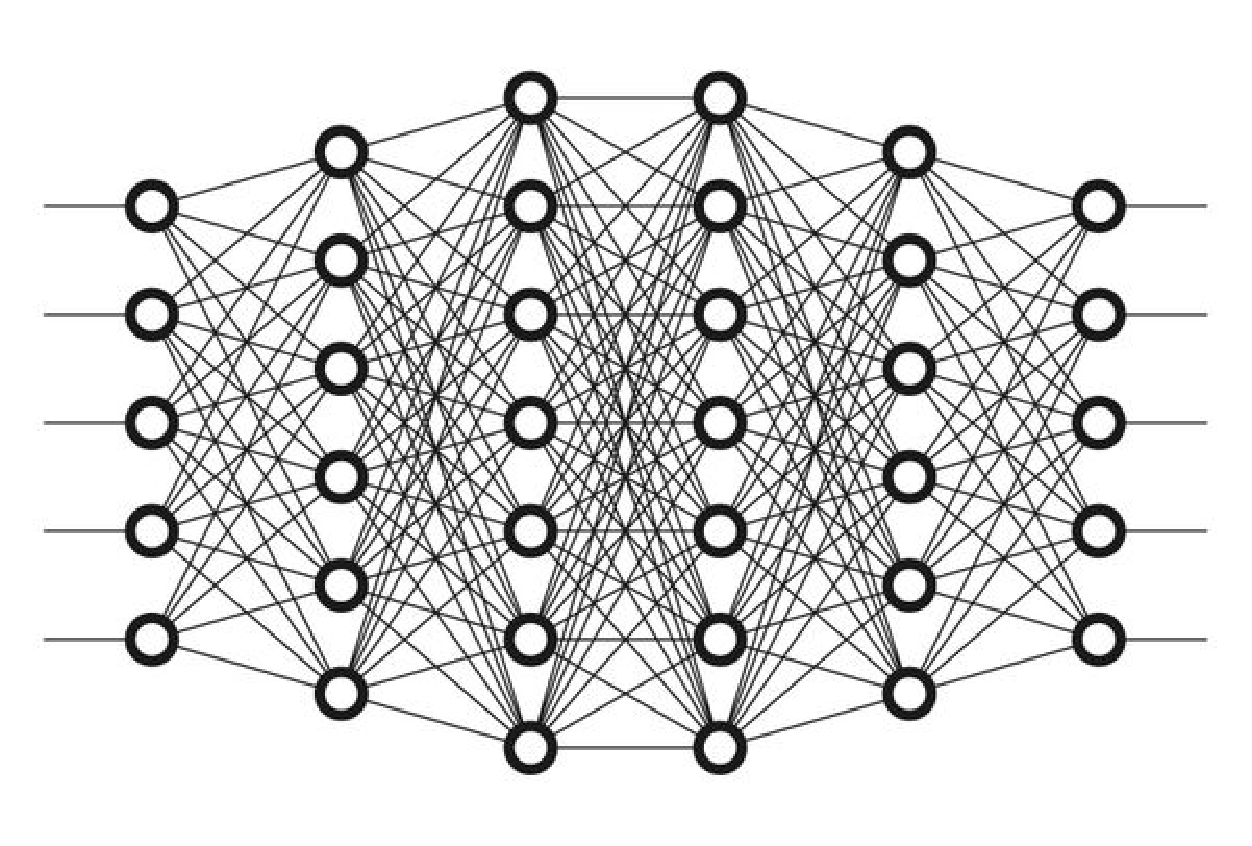
\includegraphics[width=1\textwidth,clip]{Figures/DNN.eps}
\end{figure}
}

\only<2->{
 \begin{minipage}[c]{3.5cm}
\textbf{\footnotesize MPC policy}\\ 
\vspace{-.25cm}
{\center
  $\vect\pi_{\textcolor{myGreen3}{\vect\theta}}^\mathrm{MPC}\left({\color{blue}\vect s} \right) = {\vect u^\star_{0}}$ from}
{\tiny
\begin{align*}
\min_{\vect x,\vect u}&\quad   T_{\textcolor{myGreen3}{\vect\theta}}\left(\vect x_N\right) + \sum_{k=0}^{N-1} L_{\textcolor{myGreen3}{\vect\theta}}\left(\vect x_k,\vect u_k\right)  \\
\mathrm{s.t.}&\quad \vect x_{k+1} = \vect f_{\textcolor{myGreen3}{\vect\theta}}\left(\vect x_k,\vect u_k\right)\\
&\quad  \vect h_{\textcolor{myGreen3}{\vect\theta}}\left(\vect x_k,\vect u_k\right)\leq 0,\quad \vect{x}_0 = {\color{blue}\vect s}
\end{align*}}
\vspace{-.5cm}
\end{minipage}
}

\end{overlayarea}

 };
 
\node [ID_block, right of=sys0, node distance = 4.2cm] (ID0) {
 \begin{minipage}[c]{3.5cm}
\textbf{RL}
adjusts ${\vect{\theta}}$ to achieve
\begin{align*}
\nabla_{\textcolor{myGreen3}{\vect\theta}}J\left(\vect\pi_{\textcolor{myGreen3}{\vect\theta}}^\mathrm{MPC}\right) =0
\end{align*}
\flushright from data
\end{minipage}
 };
 
\path [line] (opt0) -- node [ anchor=south] {$\vect{a}$} (sys0);
\path [line] (sys0.south)  -- ++(0,-1) -| node [ anchor=north] {${\color{blue}\vect s}$} (opt0.south);
\path [line] (sys0) -- node [ anchor=south] {$\vect{s}_+,\vect{s},\vect{a}$} (ID0);
\path [line] (ID0.north) -- ++(0,0.85) -| node [ anchor=south] {$\textcolor{myGreen3}{\vect\theta}$} (opt0.north);
 \end{tikzpicture}
 
\begin{columns}[t]
\column{0.5\textwidth}
\visible<3->{
\textbf{Why is it useful?}
\vspace{-.1cm}
\begin{itemize}
\scriptsize
\item[$\checkmark$] Tunes your optimization model for real-world performance
\item[$\checkmark$] MPC: 25 years of results on formal guarantees \& methods
\item[$\checkmark$] Easy to inject knowledge 
\item[$\checkmark$] Learning does not start from scratch
\item[$\checkmark$] Planning provides explainability
\item[$\checkmark$] Software now available
\end{itemize}
}

\column{0.5\textwidth}
\visible<4->{
\textbf{Why can it be difficult?}
\begin{itemize}
\scriptsize
\item[\ding{56}] Optimization is computationally more expensive than a DNN
\item[\ding{56}] Deployment on GPUs is lagging
\item[\ding{56}] Non-convexity can get in the way...
%\item[\ding{56}] Does not resolve ``all" RL issues
%\item[\ding{56}] Some remaining questions
\end{itemize}
}
\visible<5->{
\center
\textbf{
Generalization to combinatorial optimization / stochastic prog. is ongoing }
}
\end{columns}


\end{frame}







%\begin{frame}{\normalsize RLMPC - RL or MPC perspective?}
%\footnotesize
%
%
%\newcommand{\Sys}{\vspace{-0.25cm}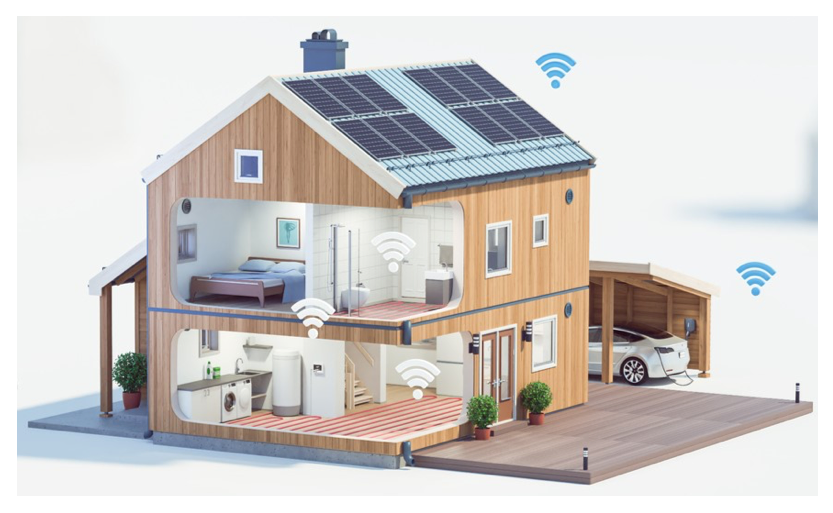
\includegraphics[width=1\textwidth,clip]{Figures/SmartHouse.eps}}
%
%\tikzstyle{Sys_block} = [rectangle, draw, fill=none,  text width=2.5cm, text centered, rounded corners, minimum height=4em,inner sep=2pt]
%\tikzstyle{Opt_block} = [rectangle, draw, fill=myLightGreen,  text width=3.5cm,  text centered, rounded corners]
%\tikzstyle{ID_block} = [rectangle, draw, fill=myLightBlue,  text width=3.5cm, text centered, rounded corners]    
%\tikzstyle{line} = [draw, -latex']
%
%\begin{tikzpicture}%[node distance = 4cm, auto]
%
%\node [Sys_block] (sys0) {\Sys};
%
%\node [Opt_block, left of=sys0, node distance = 4cm] (opt0) {
% \begin{minipage}[c]{3.5cm}
%\textbf{\footnotesize MPC policy}\\ 
%\vspace{-.2cm}
%{\center
%  $\vect\pi_{\textcolor{myGreen3}{\vect\theta}}^\mathrm{MPC}\left({\color{blue}\vect s} \right) = {\vect u^\star_{0}}$ from}
%{\tiny
%\begin{align*}
%\min_{\vect x,\vect u}&\quad   T_{\textcolor{myGreen3}{\vect\theta}}\left(\vect x_N\right) + \sum_{k=0}^{N-1} L_{\textcolor{myGreen3}{\vect\theta}}\left(\vect x_k,\vect u_k\right)  \\
%\mathrm{s.t.}&\quad \vect x_{k+1} = \vect f_{\textcolor{myGreen3}{\vect\theta}}\left(\vect x_k,\vect u_k\right)\\
%&\quad  \vect h_{\textcolor{myGreen3}{\vect\theta}}\left(\vect x_k,\vect u_k\right)\leq 0,\quad \vect{x}_0 = {\color{blue}\vect s}
%\end{align*}}
%\vspace{-.5cm}
%\end{minipage}
% };
% 
%\node [ID_block, right of=sys0, node distance = 4.2cm] (ID0) {
% \begin{minipage}[c]{3.5cm}
%\textbf{RL}
%adjusts ${\vect{\theta}}$ to achieve
%\begin{align*}
%\nabla_{\textcolor{myGreen3}{\vect\theta}}J\left(\vect\pi_{\textcolor{myGreen3}{\vect\theta}}^\mathrm{MPC}\right) =0
%\end{align*}
%\flushright from data
%\end{minipage}
% };
% 
%\path [line] (opt0) -- node [ anchor=south] {$\vect{a}$} (sys0);
%\path [line] (sys0.south)  -- ++(0,-1) -| node [ anchor=north] {${\color{blue}\vect s}$} (opt0.south);
%\path [line] (sys0) -- node [ anchor=south] {$\vect{s}_+,\vect{s},\vect{a}$} (ID0);
%\path [line] (ID0.north) -- ++(0,1) -| node [ anchor=south] {$\textcolor{myGreen3}{\vect\theta}$} (opt0.north);
% \end{tikzpicture}
% 
% \begin{columns}[t]
%\column{0.5\textwidth}
%\visible<2->{
%\textbf{RL perspective} {\tiny (MPC is ``just" a policy)}
%\begin{itemize}
%\scriptsize
%\item[$\checkmark$] MPC is a structured policy approximation
%\item[$\checkmark$] Prior knowledge are easy to embed
%\item[$\checkmark$] Handle constraints explicitly
%\item[$\checkmark$] Strong properties, solid theory
%\item[\ding{56}] MPC is expensive  {\tiny (vs. DNN)}
%\item[\ding{56}] NLP non-convexity can create issues
%\end{itemize}}
%\column{0.5\textwidth}
%\visible<3->{
%\textbf{MPC perspective} {\tiny (RL is ``just" a toolbox)}
%\begin{itemize}
%\scriptsize
%\item[$\checkmark$] RL is a toolbox for adaptive MPC
%\item[$\checkmark$] Closed-loop performance in (direct) focus
%\item[$\checkmark$] Large suit of algorithms
%\item[$\checkmark$] Not too difficult to implement
%%\item[\ding{56}] $\item[\ding{56}] Need to compute the MPC sensitivities$ is (usually) not convex%May want to solve the MPC many times on past data
%%\item[\ding{56}] Need to compute the MPC sensitivities
%\item[\ding{56}] $J$ is (usually) non-convex
%\item[\ding{56}] $\nabla_{\textcolor{myGreen3}{\vect\theta}}J$ is (usually) noisy, data intensive, can be biased
%\end{itemize}}
%\end{columns}
%
%
%
%%\begin{itemize}
%%\item Is that adaptive control? Yes but...
%%\item Highlight decoupling of learning-controlling
%%\end{itemize}
%\end{frame}

\begin{frame}{\normalsize Example - Home Energy Management {\textcolor{black}{\scriptsize(simulated)}}}
\footnotesize
\begin{columns}
\column{0.3\textwidth}
\textbf{Setup}
\vspace{-.2cm}
\begin{block}{} 
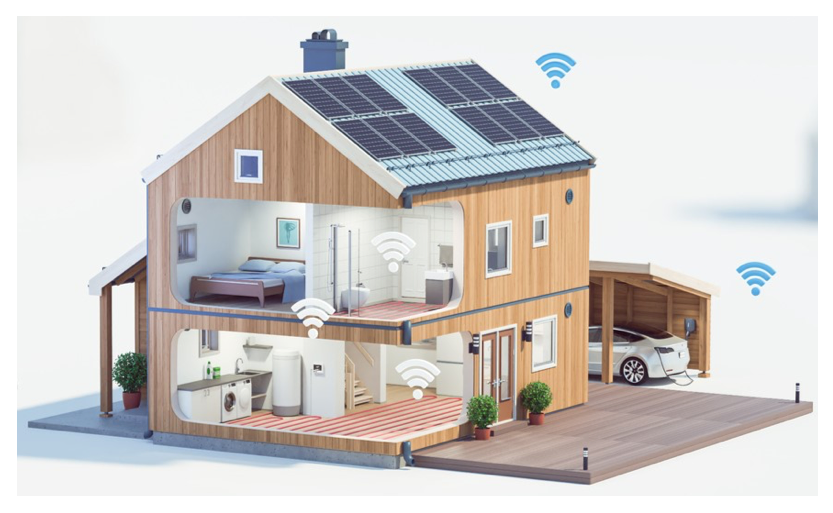
\includegraphics[width=1\textwidth,clip]{Figures/SmartHouse.eps}\\
\vspace{.25cm}
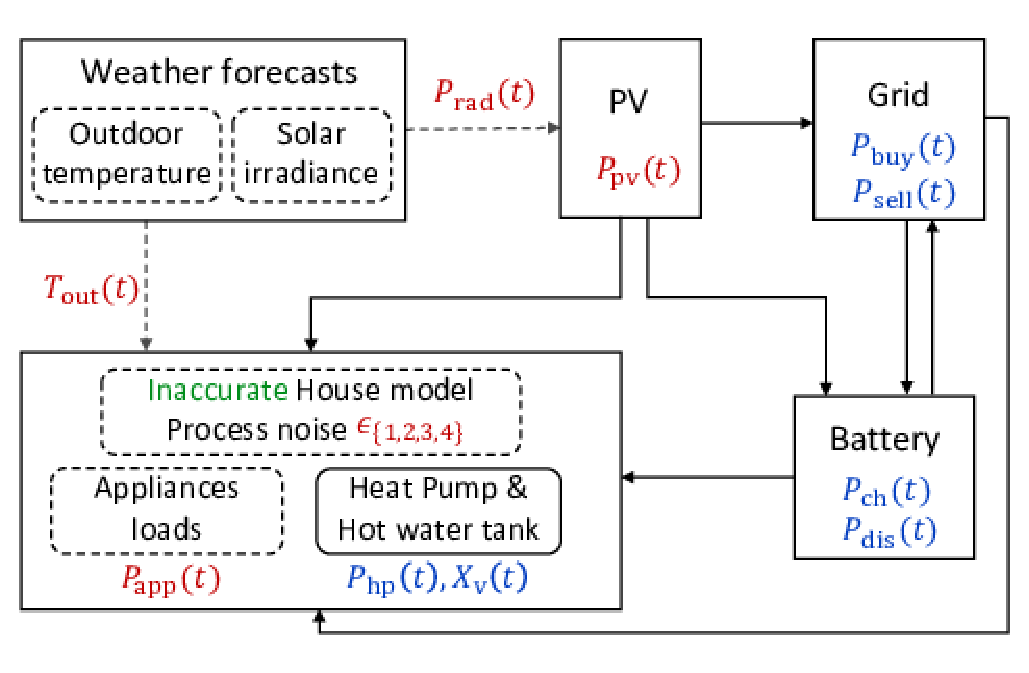
\includegraphics[width=1\textwidth,clip]{Illustration/HomeManagement/HEMS.eps}\\
\vspace{.25cm}
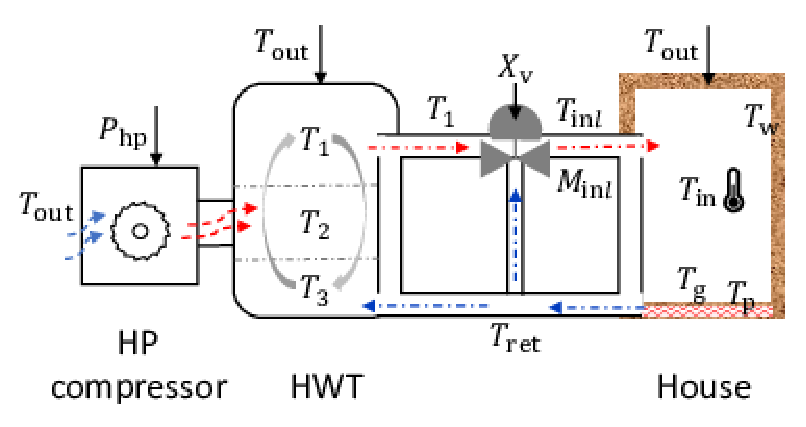
\includegraphics[width=1\textwidth,clip]{Illustration/HomeManagement/HP_HWT.eps}
\end{block} 
\column{0.65\textwidth}

\visible<2->{
\textbf{Learning process}
\tikzstyle{DATA_block} = [rectangle, draw, fill=none,  text width=2.cm, text centered, rounded corners]%, minimum height=4em,inner sep=2pt]
\tikzstyle{SYSID_block} = [rectangle, draw, fill=myLightRed,  text width=2.cm, text centered, rounded corners]%, minimum height=4em,inner sep=2pt]
\tikzstyle{RL_block} = [rectangle, draw, fill=myLightGreen,  text width=2cm,  text centered, rounded corners]
\tikzstyle{line} = [draw, -latex']

\begin{tikzpicture}%[node distance = 4cm, auto]

\node [DATA_block] (Data0) {
\vspace{-.5cm}
\center
\textbf{Real world data}
};
\visible<3->{\node [SYSID_block, right of=Data0, node distance = 3.1cm] (SYSID0) {
Classical model fitting to build MPC model
 };}
 
\visible<4->{\node [RL_block, right of=SYSID0, node distance = 2.6cm] (RL0) {
Reinforcement Learning over MPC
 };}
 
\visible<3->{\path [line] (Data0) -- node [ anchor=south] {Data} (SYSID0);}
\visible<4->{\path [line] (SYSID0) -- node [ anchor=south] {$\vect{\theta}$} (RL0);}
%\path [line] (SYSID0) -- node [ anchor=south] {$\vect{a}$} (RL0);
 \end{tikzpicture}}
 
\visible<5->{
\begin{columns}[t]
\column{0.5\textwidth}
\textbf{RL phase} {\tiny (2 RL algo.)}
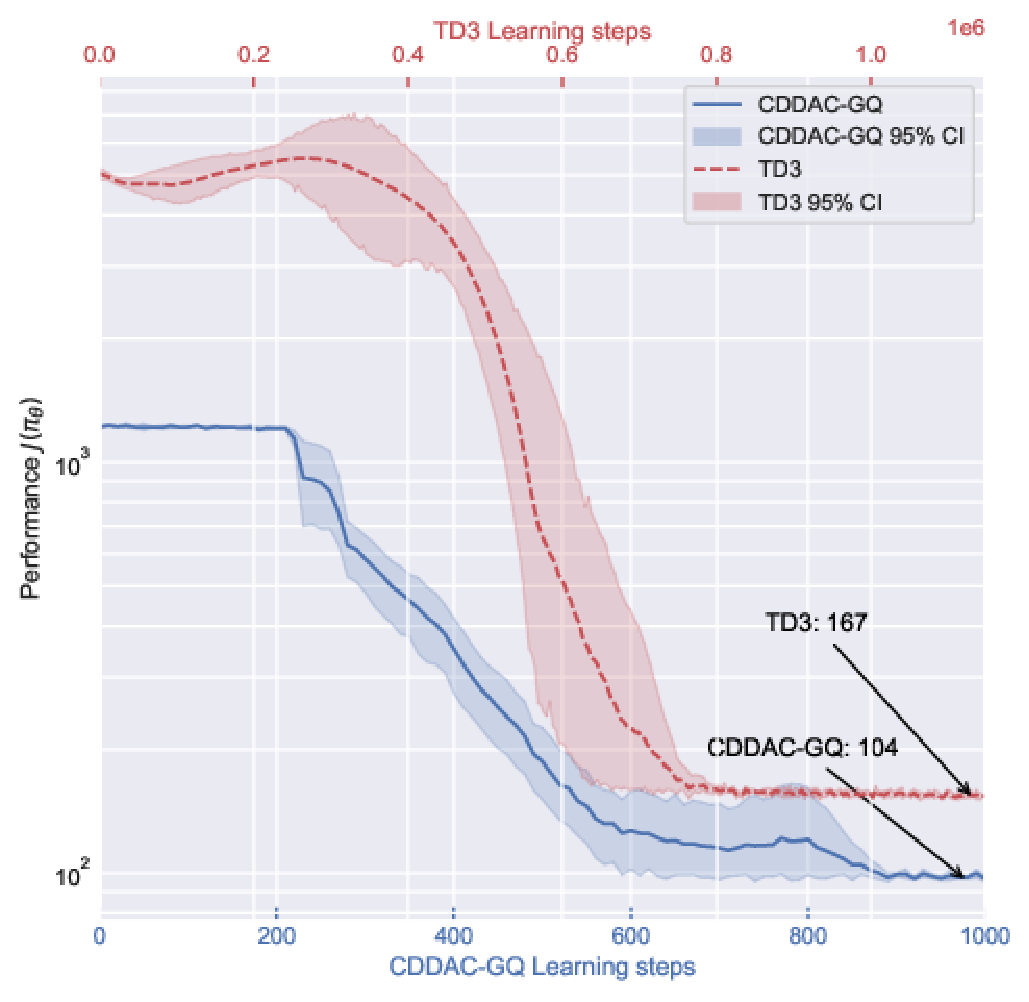
\includegraphics[width=1\textwidth,clip]{Illustration/HomeManagement/JJ-cropped.eps}}

\column{0.5\textwidth}
\visible<6->{
\begin{alertblock}{}
\center
\textbf{
The RL step improves the MPC performance significantly from only model fitting}
\end{alertblock}}
\end{columns}
\end{columns}
\end{frame}



%\begin{frame}{\normalsize Model fitting?}
%\footnotesize
%
%\begin{columns}
%\column{0.45\textwidth}
%
%\begin{overlayarea}{\textwidth}{0.45\textheight}
%
%\only<1>{
%\textbf{Proposed paradigm}
%\begin{block}{}
%Policy  $\vect\pi_{\textcolor{myGreen3}{\vect\theta}}^\mathrm{MPC}\left({\color{blue}\vect s} \right) = {\vect u^\star_{0}}$ from
%\begin{align*}
%\min_{\vect x,\vect u}&\quad   T_{\textcolor{myGreen3}{\vect\theta}}\left(\vect x_N\right) + \sum_{k=0}^{N-1} L_{\textcolor{myGreen3}{\vect\theta}}\left(\vect x_k,\vect u_k\right)  \\
%\mathrm{s.t.}&\quad \vect x_{k+1} = \vect f_{\textcolor{myGreen3}{\vect\theta}}\left(\vect x_k,\vect u_k\right)\\
%&\quad  \vect h_{\textcolor{myGreen3}{\vect\theta}}\left(\vect x_k,\vect u_k\right)\leq 0,\quad \vect{x}_0 = {\color{blue}\vect s}
%\end{align*}
%\end{block}}
%
%\only<2->{
%A step back: \textbf{model adjustment?}
%\begin{block}{}
%Policy  $\vect\pi_{\textcolor{myGreen3}{\vect\theta}}^\mathrm{MPC}\left({\color{blue}\vect s} \right) = {\vect u^\star_{0}}$ from
%\begin{align*}
%\min_{\vect x,\vect u}&\quad   T\left(\vect x_N\right) + \sum_{k=0}^{N-1} L\left(\vect x_k,\vect u_k\right)  \\
%\mathrm{s.t.}&\quad \vect x_{k+1} = \vect f_{\textcolor{myGreen3}{\vect\theta}}\left(\vect x_k,\vect u_k\right)\\
%&\quad  \vect h\left(\vect x_k,\vect u_k\right)\leq 0,\quad \vect{x}_0 = {\color{blue}\vect s}
%\end{align*}
%\end{block}
%}
%\end{overlayarea}
%
%\begin{overlayarea}{\textwidth}{0.4\textheight}
%%\only<2>{
%%\center
%%\textbf{Obvious observation:} working with model alone ``costs" us degrees of freedom. How bad is that? More in a bit.
%%}
%\only<2->{
%\textbf{Adjust ${\textcolor{myGreen3}{\vect\theta}}$ according to} (e.g.)
%\begin{align*}
%1.&\quad \min_{\textcolor{myGreen3}{\vect\theta}} \mathbb E\left[\left\|\vect f_{\textcolor{myGreen3}{\vect\theta}}\left(\vect s,\vect a\right) - \vect s_{+}\right\|^2\right]\text{ vs.} \\
%2. &\quad \min_{\textcolor{myGreen3}{\vect\theta}} J\left(\vect\pi_{\textcolor{myGreen3}{\vect\theta}}^\mathrm{MPC}\right)
%\end{align*}
%\flushright ... \textbf{is that different?}
%}
%\end{overlayarea}
%
%\column{0.5\textwidth}
%\visible<3->{
%\center
%\textbf{What model yields an optimal policy?}
%\begin{block}{}
%\textbf{Early answers:}
%\begin{itemize}
%\item In general it is different...
%\item Our experience: $1\rightarrow 2$
%\begin{itemize}
%\scriptsize
%\item Better closed-loop performance
%\item But gain varies strongly from case-to-case. What causes that?
%\end{itemize} 
%\scriptsize
%\flushright (with or without full parametrization)
%\end{itemize}}
%
%\end{block}
% 
% 
% \visible<4->{ 
% \begin{alertblock}{}
% \center
%\textbf{What can the theory tell us?}
% \end{alertblock}
% 
%} 
%\end{columns}
%
%
%
%\end{frame}
%




\begin{frame}{\normalsize}{}

\textcolor{blue}{\huge For a deeper dive...}

\begin{columns}
\column{0.425\textwidth}
\vspace{-.9cm}\\
\footnotesize
\center

%\vspace{-.25cm}

\includegraphics[width=1\textwidth,clip]{RG.eps}
\column{0.5\textwidth}

\includegraphics[width=1\textwidth,clip]{GoogleScholar.eps}
\end{columns}
\vspace{-1cm}
\begin{columns}[t]
\column{0.3\textwidth}
\center
\footnotesize
\textbf{ResearchGate}
\column{0.4\textwidth}
\center
\footnotesize
\textbf{Google Scholar}
\end{columns}


\end{frame}


\end{document}
